% ==============================================================================
% TCC - Nome do Aluno
% Capítulo 1 - Introdução
% ==============================================================================
\chapter{Introdução}
\label{sec-intro}

%Antigamente, os servidores não comportavam páginas \textit{Web} que continham um conteúdo muito denso. Funcionando apenas com páginas estáticas, realizar manutenções e controle das funcionalidades era uma tarefa muito difícil. Com o desenvolvimento de novas tecnologias a partir da criação da \textit{World Wide Web} (WWW) e através do surgimento de novas linguagens de programação para a \textit{Web}, os servidores tiveram que ser adaptados para se tornarem mais robustos. Com a infraestrutura de software modificada, os servidores começaram a aceitar páginas dinâmicas que passaram a ser carregadas de conteúdos que antes não eram suportados e isso também possibilitou que essas páginas possuíssem efeitos diversos, tais como animações de conteúdo.

Antigamente, no início da \textit{World Wide Web} (WWW), os sites eram constituídos por diversos arquivos de hipertexto lincados que apresentavam as informações através da utilização de gráficos limitados e de textos. Com o passar do tempo e com o surgimento de ferramentas de desenvolvimento, os engenheiros da internet puderam oferecer mais informações por meio da capacidade computacional. Nascendo assim, os sistemas e aplicações baseadas na \textit{Web (WebApp)}. Nos dias atuais, as \textit{WebApps} se tornaram ferramentas computacionais sofisticadas que foram integradas às aplicações de negócio e aos bancos de dados corporativos, oferecendo funções especializadas aos usuários finais~\cite{pressman:es11}.    

Com a criação de diversas \textit{WebApps} diferentes, é importante ressaltar que uma aplicação \textit{Web} pode se enquadrar em mais de uma categoria, assim como realizar uma troca de categoria ao longo do seu tempo de vida~\cite{beder:ew12}. Desta maneira, o foco deste trabalho serão os Sistemas de Informação Baseados na \textit{Web (Web-based Information Systems – WISs)}, que são enquadrados em uma categoria específica de \textit{WebApps}. Esses sistemas são caracterizados como sistemas de informação tradicionais, mas estão disponíveis na Internet.

Quando falamos sobre o desenvolvimento de \textit{WebApps} atuais, em particular os WISs, temos que entender que utilizar a Engenharia de Software é uma tarefa fundamental. Os aspectos relacionados ao estabelecimento de técnicas, processos, métodos, ferramentas e ambientes de suporte ao desenvolvimento de software são tratados de forma clara pela Engenharia de Software~\cite{falbo:es14}. Trazendo alguns benefícios como, por exemplo, a compatibilidade entre plataformas e a facilidade de gerenciamento, as \textit{WebApps}, por meio dos servidores, se tornaram indispensáveis para manterem os serviços e as aplicações disponíveis em qualquer parte do mundo através da Internet.

No meio de tantas criações e adaptações tecnológicas, surge o uso de \textit{frameworks} para \textit{WebApps}. Se tornando uma das ferramentas mais importantes para o desenvolvimento de \textit{WebApps}, os \textit{frameworks} passaram a auxiliar no encapsulamento das funcionalidades de alto nível com maior eficiência e agilidade, fazendo com que a maior parte do tempo e do trabalho fossem economizados. Visando propor uma abordagem diferenciada para a construção de sistemas para \textit{Web}, surge então o método FrameWeb (\textit{Framework-based Design Method for Web Engineering})~\cite{souza:masterthesis07,souza-celebratingfalbo20}.

Baseado na linguagem de modelagem UML (\textit{Unifield Modeling Language})~\cite{booch-et-al:u06}, o método FrameWeb propõe quatro diagramas para a fase de projeto de software que incorporam os conceitos trazidos pelos \textit{frameworks} utilizados no desenvolvimento Web, de modo a facilitar a comunicação entre desenvolvedores, agilizar o desenvolvimento por meio de geração de código, dentre outras vantagens. Originalmente, o método se propunha a dar suporte a três categorias de \textit{frameworks}: controladores frontais, injeção de dependências e mapeamento objeto/relacional.

Existem, no entanto, inúmeros \textit{frameworks} existentes dentro de cada categoria. Sendo assim, se faz necessário experimentar o método com \textit{frameworks} diversos, avaliando sua adequação. Neste contexto, \citeonline{duarte-pg14} desenvolveu uma \textit{WebApp} --- um Sistema de Controle de Afastamento de Professores (SCAP) --- em seu trabalho de conclusão de curso. Esse sistema foi criado para apoiar um departamento de universidade a realizar um controle das solicitações de afastamento de seus professores efetivos. Utilizando os requisitos que foram levantados por \citeonline{duarte-pg14} e posteriormente analisados por \citeonline{prado-pg15}, este trabalho tem com tarefa fundamental a implementação do SCAP utilizando outro \textit{framework Web}, para que seja possível realizar a verificação da eficiência do método FrameWeb.

O \textit{framework} experimentado neste trabalho será o Grails. O \textit{framework} Grails utiliza as linguagens de programação Java e Groovy, tendo como característica a minimização da complexidade da criação de \textit{WebApps} e podendo ser integrado com qualquer biblioteca Java através de plugins.

%\hrulefill

%Além do template pronto para uso, este documento inclui exemplos de uso de \latex que podem ser úteis para aqueles que possuem pouca experiência com a ferramenta. Quando for começar a escrever seu PG, apague todo o conteúdo abaixo da palavra ``Texto''.

\section{Justificativa e Motivação}
\label{sec-intro-justificativa-motivacao}

Desenvolver um sistema com o método FrameWeb, representa uma grande busca entre as diversas fontes de conhecimento envolvendo o desenvolvimento \textit{Web} e as inúmeras áreas dentro da computação. O conhecimento adquirido entre essas áreas, quando somado, estabelece um processo de aprendizagem que agrega um valor inestimável durante as fases do desenvolvimento do projeto.

O projeto também contribui no aprimoramento e no desenvolvimento do método FrameWeb, uma vez que ao experimentá-lo utilizando um novo tipo de \textit{framework}, possibilita realizar a atualização da lista de suas aplicações. Ainda neste contexto, este projeto é responsável por auxiliar o Departamento de Informática, administrando o processo de afastamento de professores, que por sua vez, pode se tornar complexo sem um meio de automatização.

Agilizar a execução deste processo possibilita que tanto os secretários quanto os professores do Departamento de Informática possam controlar as requisições e avaliações de afastamentos, diminuindo o tempo entre as etapas e anulando possíveis erros.               



%%% Início de seção. %%%
\section{Objetivos}
\label{sec-intro-objetivos}

Este trabalho tem como objetivo geral a aplicação do método FrameWeb~\cite{souza:masterthesis07,souza-celebratingfalbo20}, realizando uma nova implementação do SCAP, utilizando o \textit{framework} Grails. Uma vez que os requisitos foram levantados por \citeonline{duarte-pg14} e reformulados por \citeonline{prado-pg15}, é possível verificar como o método se comporta, apresentando a devida evolução.

O objetivo geral pode ser subdividido nos seguintes objetivos específicos:

\begin{itemize}

	\item Utilizar o \textit{framework} Grails para realizar uma nova implementação do SCAP, aproveitando os seus requisitos. Nesse objetivo será possível aplicar os conceitos de Engenharia de Requisitos, Projeto de Sistemas de Software e Engenharia de Software;
	\item Aplicar o método FrameWeb para definir a documentação da arquitetura do projeto de sistema para o \textit{framework};
    \item Realizar o estudo dos requisitos já levantados e efetuar uma comparação entre os \textit{frameworks} que já foram utilizados em versões anteriores.

\end{itemize}


%O documento é organizado em capítulos (\texttt{\textbackslash chapter\{\}}), seções (\texttt{\textbackslash section\{\}}), subseções (\texttt{\textbackslash subsection\{\}}), sub-subseções (\texttt{\textbackslash subsubsection\{\}}) e assim por diante. Atenção, porém, a não criar estruturas muito profundas (sub-sub-sub-...) pois o documento não fica bem estruturado.


\section{Método de Trabalho}
\label{sec-intro-metodo}

De acordo com a seção anterior, para que os objetivos apresentados fossem alcançados, foi necessário realizar os seguintes passos:

\begin{enumerate}

    \item Revisão bibliográfica e pesquisa: leitura dos padrões de Projeto de Sistemas de Software~\cite{falbo:pss18}, análise dos temas de Engenharia de Software~\cite{falbo:es14}, Engenharia de Requisitos~\cite{falbo:er17} e entendimento do método FrameWeb~\cite{souza:masterthesis07} para realizar a aplicação do \textit{framework} Grails;
    \item Estudo do sistema SCAP: organização das informações referentes aos requisitos levantados por \citeonline{duarte-pg14} e \citeonline{prado-pg15};
    \item Definição da documentação do projeto: através do uso do método FrameWeb, elaboração da arquitetura do projeto para o \textit{framework} utilizado;
    \item Desenvolvimento da implementação: geração de uma nova implementação do SCAP através do uso do \textit{framework} descrito no projeto; 
    \item Redação da monografia: utilização do template abnTeX\footnote{\url{https://www.abntex.net.br/}} para a escrita da monografia em \latex\footnote{\url{https://www.latex-project.org/}} seguindo os requisitos das normas da ABNT (Associação Brasileira de Normas Técnicas);
    \item Apresentação do Projeto: apresentação final da monografia e demonstração do sistema SCAP com o \textit{framework} proposto.

\end{enumerate}    


\section{Organização da Monografia}
\label{sec-intro-organizacao}


A organização desta monografia foi construída e dividida da seguinte maneira:

\begin{itemize}

\item \textbf{Capítulo \ref{sec-intro}: Introdução}

Esse capítulo descreve a metodologia utilizada, os objetivos e as questões relacionadas ao contexto do projeto. 

\item \textbf{Capítulo \ref{sec-referencial}: Referencial Teórico}

Esse capítulo descreve o que foi estudado com relação aos principais temas abordados ao longo deste trabalho, ou seja: o método FrameWeb, Engenharia \textit{Web} e \textit{Frameworks}.

\item \textbf{Capítulo \ref{sec-requisitos}: Especificação de Requisitos}

Esse capítulo traz uma breve descrição das funcionalidades e objetivos do SCAP, assim como a análise dos requisitos e especificação.

\item \textbf{Capítulo \ref{sec-projeto}: Projeto Arquitetural e Implementação}

Esse capítulo exibe o resultado da execução do método FrameWeb no projeto, trazendo os modelos e mostrando as tecnologias utilizadas na implementação. 

\item \textbf{Capítulo \ref{sec-conclusoes}: Considerações Finais}

Esse capítulo apresenta as expectativas relacionadas a trabalhos futuros e mostra as conclusões referentes à nova implementação do SCAP.  

\end{itemize}

\begin{comment}


%%% Início de seção. %%%
\subsection{Referências a seções}
\label{sec-intro-secoes-refs}



Cada parte do documento (capítulo, seção, etc.) deve possuir um rótulo logo abaixo de sua definição. Por exemplo, este capítulo é definido com \texttt{\textbackslash chapter\{Introdução\}} seguido por \texttt{\textbackslash label\{sec-intro\}}. Assim, podemos fazer referências cruzadas usando o comando \texttt{\textbackslash ref\{rótulo\}}: ``O Capítulo~\ref{sec-intro} começa com a Seção~\ref{sec-intro-secoes}, que é ainda subdividida nas subseções~\ref{sec-intro-secoes-refs} e~\ref{sec-intro-secoes-sobrerefs}.




Para melhor organização das partes do documento, sugere-se primeiro utilizar o prefixo \texttt{sec-} (para diferenciar de referências à figuras, tabelas, etc. quando usarmos o comando \texttt{\textbackslash ref\{\}}) e também representar a hierarquia das seções nos rótulos. Por exemplo, o Capítulo~\ref{sec-intro} tem rótulo \texttt{sec-intro}, sua Seção~\ref{sec-intro-secoes} tem rótulo \texttt{sec-intro-secoes} e a Subseção~\ref{sec-intro-secoes-refs} tem rótulo \texttt{sec-intro-secoes-refs}.



%%% Início de seção. %%%
\subsection{Sobre referências cruzadas}
\label{sec-intro-secoes-sobrerefs}

Nas próximas seções, veremos que é possível fazer referência cruzada não só a seções mas também a listagens de código, figuras, tabelas, etc. Em todos estes casos, quando nos referimos à Seção X, Listagem Y ou Figura Z, consideramos que estes são os nomes próprios destes elementos e, portanto, usa-se a primeira letra maiúscula. Isso pode ser visto na Subseção~\ref{sec-intro-secoes-refs}, acima. A exceção é quando nos referimos a vários elementos ao mesmo tempo, por exemplo: ``as subseções~\ref{sec-intro-secoes-refs} e~\ref{sec-intro-secoes-sobrerefs}''.

Por fim, ao usar o comando \texttt{\textbackslash ref\{\}}, sugere-se separá-lo da palavra que vem antes dele com um \textasciitilde\ ao invés de espaço. Por exemplo: \texttt{o capítulo\textasciitilde \textbackslash ref\{sec-intro\}}. Isso faz com que o \latex não quebre linha entre a palavra \texttt{capítulo} e o número do capítulo.




%%% Início de seção. %%%
\section{Citações bibliográficas}
\label{sec-intro-citacoes}

Este documento utiliza a ferramenta de gerenciamento de referências bibliográficas do \latex, chamada \emph{BibTeX}. O arquivo \texttt{bibliografia.bib}, referenciado no arquivo \latex principal deste documento, contém algumas referências bibliográficas de exemplo. Assim como capítulos, seções, etc., tais referências também possuem rótulos, especificados como primeiro parâmetro de cada entrada (ex.: \texttt{@incollection\{souza-et-al:iism08, ...\}}.

Sugere-se um padrão para rótulos de referências bibliográficas para que fique claro também no código \latex qual referência está sendo citada. Por exemplo, ao citar a referência \texttt{souza-et-al:sesas13}, sabemos que é um artigo escrito por \emph{Souza} e outros, publicado no \emph{SESAS} em \emph{2013} (geralmente a pessoa que citou sabe que publicação é SESAS e quem é Souza).

Para citar uma referência bibliográfica contida no arquivo \emph{BibTeX}, basta usar seu rótulo como parâmetro de um de dois comandos possíveis de citação:

\begin{itemize}
	\item O comando \texttt{\textbackslash cite\{\}} efetua uma citação tradicional, colocando o nome do(s) autor(es) e o ano entre parênteses. Por exemplo, \texttt{\textbackslash cite\{souza-et-al:iism08\}} é transformado em~\cite{souza-et-al:iism08};
	
	\item O comando \texttt{\textbackslash citeonline\{\}} efetua uma citação integrada ao texto, colocando o nome do(s) autor(es) direto no texto e somente o ano entre parênteses. Por exemplo, ``de acordo com \texttt{\textbackslash citeonline\{souza-et-al:iism08\}}'' é transformado em: de acordo com \citeonline{souza-et-al:iism08};
\end{itemize}

Também é possível citar vários trabalhos de uma só vez, separando os rótulos das referências bibliográficas com uma vírgula dentro do comando apropriado. Por exemplo, \texttt{\textbackslash cite\{souza-et-al:sesas13,souza-et-al:csrd13\}}~\cite{souza-et-al:sesas13,souza-et-al:csrd13}.

Os trabalhos citados são automaticamente incluídos na seção de referências bibliográficas, ao final do documento. Tudo é formatado automaticamente segundo padrões da ABNT.



%%% Início de seção. %%%
\section{Listagens de código}
\label{sec-intro-listagens}

O pacote \texttt{listings}, incluído neste template, permite a inclusão de listagens de código. Análogo ao já feito anteriormente, listagens possuem rótulos para que possam ser referenciadas e sugerimos uma regra de nomenclatura para tais rótulos: usar como prefixo o rótulo do capítulo, substituindo \texttt{sec-} por \texttt{lst-}.

A Listagem~\ref{lst-intro-exemplo}, por exemplo, possui o rótulo \texttt{lst-intro-exemplo} e representa o código que foi usado no próprio documento para exibir as listagens desta seção. Como podemos ver, a sugestão é que os arquivos de código sejam colocados dentro da pasta \texttt{codigos/} e tenham nome idêntico ao rótulo, colocando a extensão adequada ao tipo de código.

\lstinputlisting[label=lst-intro-exemplo, caption=Exemplo de código \latex para inclusão de listagens de código., float=htpb]{codigos/lst-intro-exemplo.tex}

A Listagem~\ref{lst-intro-outroexemplo} mostra um exemplo de listagem com especificação da linguagem utilizada no código. O pacote \texttt{listings} reconhece algumas linguagens\footnote{Veja a lista de linguagens suportadas em \url{http://en.wikibooks.org/wiki/LaTeX/Source\_Code\_Listings\#Supported_languages}.} e faz ``coloração'' de código (na verdade, usa \textbf{negrito} e não cores) de acordo com a linguagem. O parâmetro \texttt{float=htpb} incluído em ambos os exemplos impede que a listagem seja quebrada em diferentes páginas.

\lstinputlisting[label=lst-intro-outroexemplo, caption=Exemplo de código \java especificando linguagem utilizada., language=Java, float=htpb]{codigos/lst-intro-outroexemplo.java}



%%% Início de seção. %%%
\section{Figuras}
\label{sec-intro-figuras}

Figuras podem ser inseridas no documento usando o \emph{ambiente} \texttt{figure} (ou seja, \texttt{\textbackslash begin\{figure\}} e \texttt{\textbackslash end\{figure\}}) e o comando \texttt{\textbackslash includegraphics\{\}}. Existem alguns outros elementos e propriedades úteis de serem configuradas, resultando no código exibido na Listagem~\ref{lst-intro-figuras}.

\lstinputlisting[label=lst-intro-figuras, caption=Código \latex utilizado para inclusão das figuras na Seção~\ref{sec-intro-figuras}., float=htpb]{codigos/lst-intro-figuras.tex}

O comando \texttt{\textbackslash centering} centraliza a figura na página. A opção \texttt{width} do comando \texttt{\textbackslash includegraphics\{\}} determina o tamanho da figura e usa-se \texttt{\textbackslash textwidth} (opcionalmente multiplicado por um número) para se referir à largura da página.

O parâmetro do comando \texttt{\textbackslash includegraphics\{\}} indica onde a imagem pode ser encontrada. Foi criado o diretório \texttt{figuras/} para conter as figuras do documento, dando uma melhor organização aos arquivos. Ao abrir esta pasta, repare que as figuras possuem duas versões---uma em \texttt{.eps} e outra em \texttt{.pdf}---e que o comando \texttt{\textbackslash includegraphics\{\}} não especifica a extensão. Isso se dá porque o \latex possui um compilador para formato PostScript (\texttt{latex}) que espera as imagens em \texttt{.eps} e um compilador para PDF (\texttt{pdflatex}) que espera as imagens em \texttt{.pdf}. Dependendo do seu ambiente \latex, é possível apenas colocar as figuras em formatos mais comuns, como JPG ou PNG e ele incluir no PDF sem problemas. Vale a pena testar.

Por fim, o comando \texttt{\textbackslash caption\{\}} especifica a descrição da figura e \texttt{\textbackslash label\{\}}, como de costume, estabelece um rótulo para permitir referência cruzada de figuras. Note ainda que é utilizada a mesma estratégia de nomenclatura de rótulos usada nas listagens, porém utilizando o prefixo \texttt{fig-}.

As figuras~\ref{fig-intro-nemologo} e~\ref{fig-intro-exemplosideways} mostram o resultado do código da Listagem~\ref{lst-intro-figuras}. A Figura~\ref{fig-intro-exemplosideways}, em particular, utiliza o pacote \texttt{rotating} para mostrar figuras largas em modo paisagem. Basta usar o ambiente \texttt{sidewaysfigure} ao invés de \texttt{figure}.

\begin{figure}
	\centering
	
\includegraphics[width=.25\textwidth]{figuras/fig-intro-nemologo} 
	\caption{Exemplo de figura: logo do Nemo.}
	\label{fig-intro-nemologo}
\end{figure}

\begin{sidewaysfigure}
	\centering
	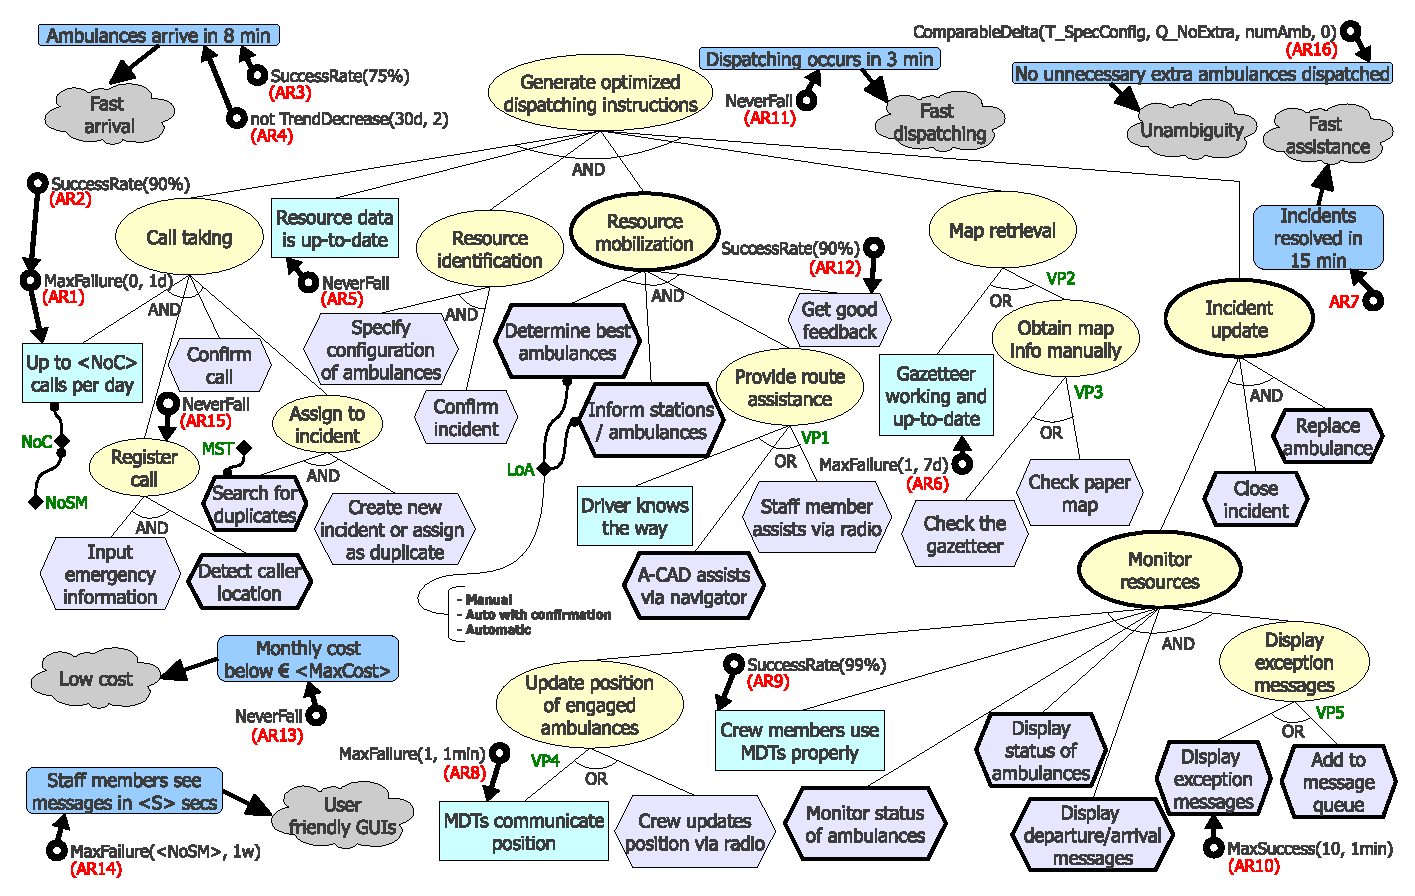
\includegraphics[width=\textwidth]{figuras/fig-intro-exemplosideways} 
	\caption{Exemplo de figura em modo paisagem: um modelo de objetivos~\cite{souza-mylopoulos:spe13}.}
	\label{fig-intro-exemplosideways}
\end{sidewaysfigure}



%%% Início de seção. %%%
\section{Tabelas}
\label{sec-intro-tabelas}

Tabelas são um ponto fraco do \latex. Elas são complicadas de fazer e, dependendo da complexidade da tabela (muitas células mescladas, por exemplo), vale a pena construi-las em outro programa (por exemplo, em seu editor de texto favorito) e inclui-las no documento como figuras. Mostramos, no entanto, alguns exemplos de tabela a seguir. O código utilizado para criar as tabelas encontra-se nas listagens~\ref{lst-intro-tabelas01}, \ref{lst-intro-tabelas02} e~\ref{lst-intro-tabelas03}.

\lstinputlisting[label=lst-intro-tabelas01, caption=Código \latex utilizado para inclusão das tabelas~\ref{tbl-intro-exemplo01} e~\ref{tbl-intro-exemplo02}., float=htpb]{codigos/lst-intro-tabelas01.tex}

\lstinputlisting[label=lst-intro-tabelas02, caption=Código \latex utilizado para inclusão da Tabela~\ref{tbl-intro-exemplo03}., float=htpb]{codigos/lst-intro-tabelas02.tex}

\lstinputlisting[label=lst-intro-tabelas03, caption=Código \latex utilizado para inclusão da Tabela~\ref{tbl-intro-exemplo04}., float=htpb]{codigos/lst-intro-tabelas03.tex}

Em particular, a Tabela~\ref{tbl-intro-exemplo04} utiliza um pacote chamado \texttt{tabularx}, que permite maior controle do layout das tabelas. Ao definir o ambiente \texttt{\textbackslash begin\{tabularx\}}, são definidos os tamanhos de cada coluna proporcional à largura ocupada pela tabela. Veja na Listagem~\ref{lst-intro-tabelas03} que as primeiras duas colunas não definem o atributo \texttt{\textbackslash hsize}, o que faz com que elas fiquem com o tamanho padrão de coluna, que é a largura da tabela dividida pelo número de colunas. Já a terceira coluna define \texttt{\textbackslash hsize=1.2\textbackslash hsize}, ou seja, esta coluna deve ser 20\% maior do que o tamanho padrão. Para isso, é preciso retirar de outras colunas, portanto a quarta e quinta colunas são definidas como 10\% menores (ou seja, \texttt{\textbackslash hsize=0.9\textbackslash hsize}).

% Exemplo de tabela 01:
\begin{table}
	\caption{Exemplo de tabela com diferentes alinhamentos de conteúdo.}
	\label{tbl-intro-exemplo01}
	\centering
	\begin{tabular}{ | c | l | r | p{40mm} |}\hline
		\textbf{Centralizado} & \textbf{Esquerda} & \textbf{Direita} & \textbf{Parágrafo}\\\hline
		C & L & R & Alinhamento de tipo parágrafo especifica largura da coluna e quebra o texto automaticamente.\\
		\hline
		Linha 2 & Linha 2 & Linha 2 & Linha 2\\
		\hline
	\end{tabular}
\end{table}

% Exemplo de tabela 02:
\begin{table}
	\caption{Exemplo que especifica largura de coluna e usa lista enumerada (adaptada de~\cite{souza-mylopoulos:spe13}).}
	\label{tbl-intro-exemplo02}
	\centering
	\renewcommand{\arraystretch}{1.2}
	\begin{small}
		\begin{tabular}{ | p{15mm} | p{77mm} | p{55mm} |}\hline
			\textbf{\textit{AwReq}} & \textbf{Adaptation strategies} & \textbf{Applicability conditions}\\\hline
			
			AR1 &
			\vspace{-2mm}\begin{enumerate}[topsep=0cm, partopsep=0cm, itemsep=0cm, parsep=0cm, leftmargin=0.5cm]
				\item \textit{Warning(``AS Management'')}
				\item \textit{Reconfigure($\varnothing$)}
			\end{enumerate}\vspace{-4mm} &
			\vspace{-2mm}\begin{enumerate}[topsep=0cm, partopsep=0cm, itemsep=0cm, parsep=0cm, leftmargin=0.5cm]
				\item Once per adaptation session;
				\item Always.
			\end{enumerate}\vspace{-4mm}
			\\\hline
			
			AR2 &
			\vspace{-2mm}\begin{enumerate}[topsep=0cm, partopsep=0cm, itemsep=0cm, parsep=0cm, leftmargin=0.5cm]
				\item \textit{Warning(``AS Management'')}
				\item \textit{Reconfigure($\varnothing$)}
			\end{enumerate}\vspace{-4mm} &
			\vspace{-2mm}\begin{enumerate}[topsep=0cm, partopsep=0cm, itemsep=0cm, parsep=0cm, leftmargin=0.5cm]
				\item Once per adaptation session;
				\item Always.
			\end{enumerate}\vspace{-4mm}
			\\\hline
		\end{tabular}
	\end{small}
\end{table}

% Exemplo de tabela 03:
\begin{table}
	\caption{Exemplo que mostra equações em duas colunas (adaptada de~\cite{souza-mylopoulos:spe13}).}
	\label{tbl-intro-exemplo03}
	\centering
	\vspace{1mm}
	\fbox{\begin{minipage}{.98\linewidth}
			\begin{minipage}{0.51\linewidth}
				\vspace{-4mm}
				\begin{eqnarray}
				\Delta \left( I_{AR1} / NoSM \right) \left[ 0, maxSM \right] > 0\\
				\Delta \left( I_{AR2} / NoSM \right) \left[ 0, maxSM \right] > 0\\
				\Delta \left( I_{AR3} / LoA \right) < 0\\
				\end{eqnarray}
				\vspace{-6mm}
			\end{minipage}
			\hspace{2mm}
			\vline 
			\begin{minipage}{0.41\linewidth}
				\vspace{-4mm}
				\begin{eqnarray}
				\Delta \left( I_{AR11} / VP2 \right) < 0\\
				\Delta \left( I_{AR12} / VP2 \right) > 0\\
				\Delta \left( I_{AR6} / VP3 \right) > 0\\
				\end{eqnarray}
				\vspace{-6mm}
			\end{minipage}
	\end{minipage}}
\end{table}

% Exemplo de tabela 04:
\begin{table}[h]
	\caption{Exemplo que utiliza o pacote \texttt{tabularx}, extraído de um artigo ainda não publicado.}
	\label{tbl-intro-exemplo04}
	\centering\tiny\def\tabularxcolumn#1{m{#1}}
	\begin{tabularx}{\columnwidth}{ >{\centering}X | >{\centering}X | >{\hsize=1.2\hsize\centering}X | >{\hsize=0.9\hsize\centering}X | >{\hsize=0.9\hsize\centering\arraybackslash}X }
		\hline
		\textbf{Applied Criteria} & \textbf{Analyzed Content} & \textbf{Initial\\Occurrences} & \textbf{Final Results} & \textbf{Reduction (\%)} \\
		\hline
		Duplicate Removal & Title, authors and year & 903 & 420 & 54,84\% \\ 
		\hline 
		IC and ECs & Title, abstract and keywords & 420 & 130 & 69,05\% \\ 
		\hline 
		IC and ECs & Full text & 130 & 117 & 10\% \\ 
		\hline 
		Final Results & -- & 903 & 117 & 87,04\% \\ 
		\hline 
	\end{tabularx}
\end{table}


\end{comment}